\documentclass{article}
\usepackage{booktabs}
\usepackage{graphicx}

\title{Biol 461 Winter 2021 TA Section 02/12/21}
\author{}
\date{}

\begin{document}

\maketitle
\section{}
We talked in class about how Parkinson's and Huntington's are, in a way, opposites. Parkinson's patients can have difficulty initiating movements, whereas Huntington's patients can have uncontrolled movement of their limbs. Parkinson's is an imbalance favoring the indirect pathway whereas Huntington's is an imbalance favoring the direct pathway. Based on these observations, make a reasonable hypothesis regarding what role D$_1$SPNs have in movement and what role D$_2$SPNs have in movement.

\section{}

Figures taken from Kravitz et al. [2010] Nature 466:622-626
\\\\Scientists specifically expressed channelrhodopsin (Chr2) in either D$_1$SPNs or D$_2$SPNs in the striatum (Str). They stimulated these neurons with a lazer and recorded the resulting neuron activity in the substantia nigra, as seen in the schematic below:\\
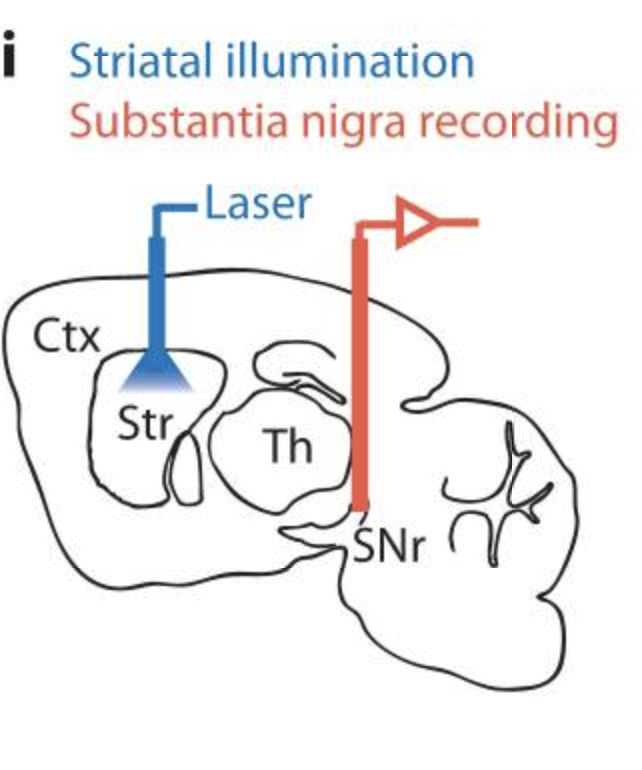
\includegraphics[scale = .5]{1.1}\\
\\ The following figure shows the resulting neural activity (the blue bar spans the time when the laser was on, the top part of the graphs show the recorded spike trains recorded with each row representing a trial and the bottom part of the graph quantifies the spike rate in Hz at each time point):\\
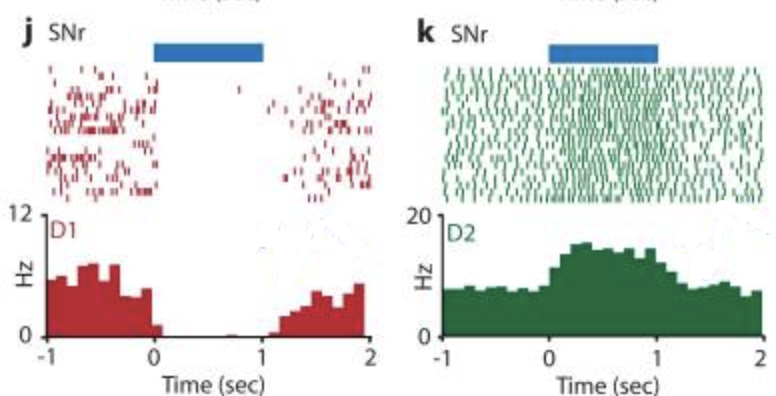
\includegraphics[scale = .8]{1.2}\\
\\\textbf{QUESTION:} Based on what you know about these neurons, what do you think the mice from above were doing during the above recordings? Provide an answer for the red mice and the green mice. Do these predictions align with your hypothesis from question 1?:\\



\section{ }
Figures taken from Klaus et al. [2017] Neuron 95:1171-1180
\\\\The following figure is a schematic of a different experiment. Calcium activity of transgenic mice expressing the fluorescent calcium reporter GCaMP6 in either their D$_1$SPNs or D$_2$SPNs was recorded using a head mounted microscope (the blue tube in B below). Mice were allowed to behave freely in a box (A below):\\
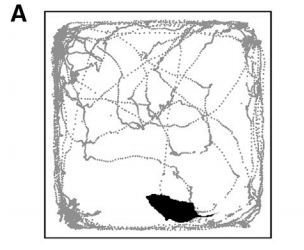
\includegraphics[]{2.1.png} 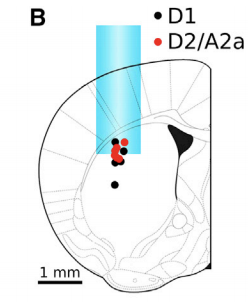
\includegraphics[]{2.2}\\
Below is a plot that shows the change in fluorescence from baseline observed in each cell population whenever the mouse initiated movement (the short bars depict a time-shifted control).\\\\
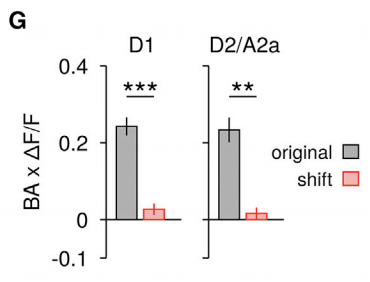
\includegraphics[]{2.3.png}\\\\
\textbf{QUESTION} Which neuron populations are involved with the initiation of movement? Do these data align with your hypothesis from question 1?

\end{document}
